Die Aufgabe der Evaluationskomponente ist es, Effizienz und Effektivität zu monitoren.
Dafür muss eine Aufzeichnung des Nutzerverhaltens sowie ausgewählter Systemmetriken vorgenommen werden.

Insbesondere zur Aufzeichnung des Nutzerverhaltens ist eine Identifikation der Nutzer notwendig.
Darauf aufbauend kann protokolliert werden, welcher Nutzer welche Anfragen ausgeführt
hat, welche Ergebnisseiten oder Query-Suggestions einem Nutzer präsentiert wurden,
sowie gegebenenfalls welche Ergebnisse oder Query Suggestions ausgewählt
wurden\footnote{Das erweitern dieser Informationen um die entsprechenden Event-Zeitpunkte erlaubt eine
sinnvolle Rekonstruktion des Nutzerverhaltens.}.

Bei einer technischen Realisierung dieser Punkte fällt auf,
dass es sich um sogenannte \href{https://de.wikipedia.org/wiki/Cross-Cutting_Concern}{Cross-Cutting Concerns}
handelt. Ein bewährtes Mittel derartige Funktionalitäten zu realisieren, ohne die
Komplexität der betroffenen Systemteile unnötig zu ehöhen,
stellt die Aspektorientierte Programmierung\footnote{AOP} dar\cite{spring.chap1.1}.
Die darin verwendeten Aspekte definieren,
was\footnote{In der zugehörigen AOP Terminologie definiert der zu einem Aspekt gehörende Advice die Aufgabe,
also was von dem Aspekt zu erledigen ist~\cite{spring.chap4.1}.}, wann\footnote{Der Advice eines Aspekts definiert 
neben dem was auch zu welchen Zeitpunkten ein Aspekt auszuführen ist.
Unter anderem kann vor, nach, oder das wrappen einer Zielmethode spezifiziert werden\cite{spring.chap4.1}.}
und wo\footnote{Durch sogenannte Pointcuts werden eine oder mehrere Methoden definiert,
an die der Advice gewoben wird\cite{spring.chap4.1}.} auszuführen ist\cite{spring.chap4.1}.

In dem für die Interaction-Komponente verwendeten Framework werden alle Endpunkte über speziell anotierte Methoden
bereitgestellt.
Diesen ist gemein, dass sie ein
\href{https://de.wikipedia.org/wiki/Plain_Old_Java_Object}{POJO}\footnote{Diese sind 
entsprechend einer gewählten Konvention in dem 
\href{https://github.com/mam10eks/search-homepage-of-university-leipzig/tree/master/search-engine-backend}{Backend-Modul}
in zugehörigen \href{https://de.wikipedia.org/wiki/Transferobjekt}{dto} Paketen definiert.}
als Model für die Antwort zurückgeben. 
Dieses Modell wird je nach Endpunkt später in ein HTML-Template\footnote{Spezifiziert innerhalb des 
\href{https://github.com/mam10eks/search-homepage-of-university-leipzig/tree/master/search-engine-backend/src/main/resources/templates}
{templates-Ordner in dem Backend-Modul}.} gerendert oder
JSON-serialisiert.

Unter diesen Vorraussetzungen eignen sich diese Methoden hervorragend,
um sie durch Aspekte um die gewünschten Funktionalitäten zu erweitern\footnote{Schließlich lassen
sie sich eindeutig und generisch über die notwendigen Endpunkt-Anotationen
identifizieren.}.
Dazu wird ein Effizienz-, ein User-Identification-, sowie ein Logging-Aspekt eingesetzt.
Der Effizienz-Aspekt misst dabei Beispielhaft für weitere Systemmetriken die Bearbeitungszeit von Anfragen,
und erweitert das zurückgegebene Model entsprechend.
Der User-Identification-Aspekt stellt
vor dem Aufruf jeder Endpunkt-Methode sicher, dass der Request mit einer
eindeutigen Identifikation des Nutzers versehen ist.
Dies wird über einen Cookie realisiert.
Der Logging-Aspekt protokolliert ausnahmslos alle verfügbaren Informationen.
Dazu notiert er für jeden Endpunkt den Request des Clients zusammen mit dem zurückzugebenden
POJO-Model\footnote{Mit diesem Vorgehen lassen sich alle angesprochenen Informationen zur Rekonstruktion des Nutzer-Verhaltens erheben,
da insbesondere die Links zu den Dokumenten auf dem Server durch Weiterleitungen aufgelöst werden.}.

Die vom Logging-Aspekt protokollierten Informationen können sowohl
Online\footnote{Beispielhaft wurde das im Rahmen dieser Arbeit für die Query-Suggestions vorgenommen.},
als auch Offline analysiert werden.
Um beides zu ermöglichen, wurde mit \href{https://kafka.apache.org/}{Apache Kafka}
eine Streaming Platform mit der Möglichkeit zur persistenten Datenhaltung~\cite{kafka.foreword} eingesetzt.
Dazu publisht der Logging-Aspekt seine Daten als Events nach Kafka.
Um diesen Logging-Aspekt so einfach wie möglich zu halten, bereitet ein
\href{https://www.confluent.io/blog/introducing-kafka-streams-stream-processing-made-simple/}{Stream Processor}
diese Daten weiter auf\footnote{Dieser Stream Processor reichert die Events an und leitet sie
auf sinnvolle Topics um. Der Quellcode ist in dem Modul 
\href{https://github.com/mam10eks/search-homepage-of-university-leipzig/tree/master/search-engine-kafka-streams}
{search-engine-kafka-streams} enthalten.}.
Online-Analysen wie die Query-Suggestion können sich nun unmittelbar an die für sie interessanten Events subscriben.
Offline Analysen können die persistierten Events gleichzeitig in einem  Batch-Vorgang verarbeiten.
Als Beispiel dafür stellt Abbildung~\ref{fig:visualization} einen mit Python realisierten
Import\footnote{Der Quellcode ist in dem Modul
\href{https://github.com/mam10eks/search-homepage-of-university-leipzig/tree/master/visualize_events}{visualize\_events}.}
der Events nach \href{https://de.wikipedia.org/wiki/Neo4j}{Neo4j} zur Visualisierung dar.

\begin{figure}[!ht]
	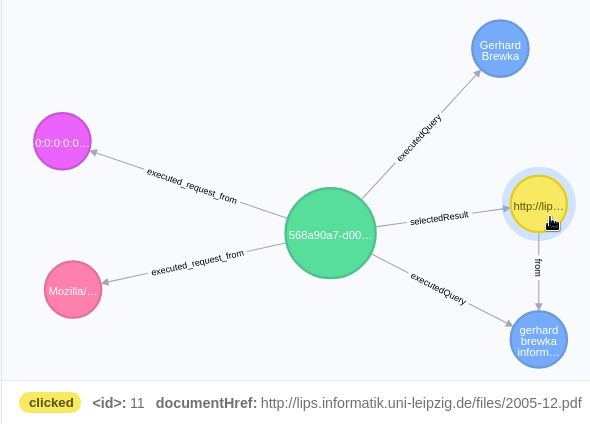
\includegraphics[width=0.99\textwidth]{chapter_query_processing/example_neo4j_visualization.png}
	\caption{Beispielgraph im
	\href{https://neo4j.com/developer/guide-neo4j-browser/}{Neo4j-Browser}
	einer User-Session bestehend aus 2 Anfragen, bei denen bei einer Anfrage ein Ergebniss angeklickt wurde.}
	\label{fig:visualization}
\end{figure}

Die hier vorgestellte Evaluationskomponente funktioniert für alle Clients, welche Cookies erlauben und den \href{}{Referrer-Header}
korrekt setzen.
